\documentclass{beamer}

\mode<presentation>
{
  \usetheme{Wolfenbuettel}
  \setbeamercovered{transparent}
}


\usepackage{pgf,pgfarrows,pgfnodes}
\usepackage[english]{babel}
\usepackage{amsmath}

\usepackage[latin1]{inputenc}

%\usepackage{times}
\usepackage{ae}
\usepackage[T1]{fontenc}
\usepackage{euler}

\usepackage{jkmath}
%\usepackage{pb-diagram}
\usepackage{fp}
\usepackage{multido}

\definecolor{MyBlue}{rgb}{0.3,0.3,1.0} 
\definecolor{MyGreen}{rgb}{0.3,1.0,0.3} 
\definecolor{MyRed}{rgb}{1.0,0.3,0.3} 

\newcommand{\textarrowdown}[1]
{
        \begin{pgfpicture}{0cm}{0cm}{4cm}{0.7cm} 
          \pgfsetlinewidth{1.0pt}
          \color{structure}
          \pgfsetendarrow{\pgfarrowto}
          \pgfline{\pgfxy(2,0.5)}{\pgfxy(2,0.0)} 
           \pgfputat{\pgfxy(2.4,0.35)}{\pgfbox[left,center]{#1}}
        \end{pgfpicture}
}
\newcommand{\textarrowup}[1]
{
        \begin{pgfpicture}{0cm}{0cm}{4cm}{0.7cm} 
          \pgfsetlinewidth{1.0pt}
          \color{structure}
          \pgfsetendarrow{\pgfarrowto}
          \pgfline{\pgfxy(2,0.0)}{\pgfxy(2,0.5)} 
           \pgfputat{\pgfxy(2.4,0.35)}{\pgfbox[left,center]{#1}}
        \end{pgfpicture}
}

\newcounter{countdy}
\newcommand{\ftriangle}[6]
{
  \newcommand{\starty}{#2}
  \setcounter{countdy}{1}
  \multido{\rx=#1+#3}{#5}
  {
    \multido{\ry=\starty+#4}{\value{countdy}}
    {
      \pgfnodecircle{Node1}[fill]{\pgfxy(\rx,\ry)}{#6} 
    }
    \FPsub{\starty}{#3}{\starty}
    \stepcounter{countdy}
    \stepcounter{countdy}
  }
}

\newcommand{\faxes}[8]
{
  \FPsub{#3}{#1}{\hx}
  \FPsub{#4}{#2}{\hy}
  \FPmul{\hx}{0.5}{\hx}
  \FPmul{\hy}{0.5}{\hy}
  \FPadd{\hx}{#1}{\hx}
  \FPadd{\hy}{#2}{\hy}
  \pgfsetendarrow{\pgfarrowto}
  \pgfline{\pgfxy(#1,\hy)}{\pgfxy(#3,\hy)} 
  \pgfline{\pgfxy(\hx,#2)}{\pgfxy(\hx,#4)} 
  \FPadd{#3}{#5}{\nx}
  \FPadd{#4}{#6}{\ny}
  \pgfputat{\pgfxy(\nx,\hy)}{\pgfbox[left,center]{#7}}
  \pgfputat{\pgfxy(\hx,\ny)}{\pgfbox[center,bottom]{#8}}
}

\newcommand{\frect}[7]
{
  \multido{\rx=#1+#3}{#5}
  {
    \multido{\ry=#2+#4}{#6}
    {
      \pgfnodecircle{Node1}[fill]{\pgfxy(\rx,\ry)}{#7} 
    }
  }
}
\setbeamertemplate{title page}
{ 
  \begin{centering}
    \begin{beamercolorbox}[sep=8pt,center,colsep=-4bp,rounded=true,shadow=true]{title}
      \usebeamerfont{title}\inserttitle\par
      \vskip0.25em           
      {\usebeamerfont{subtitle}\usebeamercolor[fg]{subtitle}\insertsubtitle\par}
    \end{beamercolorbox}
    \begin{beamercolorbox}[sep=8pt,center,colsep=-4bp,rounded=true,shadow=true]{author}
      \usebeamerfont{author}\insertauthor
    \end{beamercolorbox}
    \begin{beamercolorbox}[sep=8pt,center,colsep=-4bp,rounded=true,shadow=true]{date}
      \usebeamerfont{date}\insertdate
    \end{beamercolorbox}\vskip0.5em
  \end{centering}  
}


\title{Nonequispaced Fast Spherical Fourier Transform and Applications}

\author
{Jens Keiner}

%\institute[Universit�t zu L�beck]
%{Institut f�r Mathematik}

%\date[Oberseminar]{Oberseminar Mathematik, 29.06.2005}

%\subject{Numerical Analysis}

% If you have a file called "university-logo-filename.xxx", where xxx
% is a graphic format that can be processed by latex or pdflatex,
% resp., then you can add a logo as follows:

%\pgfdeclareimage[height=0.5cm]{university-logo}{gridsphere}
%\logo{\pgfuseimage{university-logo}}


% Delete this, if you do not want the table of contents to pop up at
% the beginning of each subsection:
\AtBeginSection[]
{
  \begin{frame}<beamer>
    \frametitle{Outline}
    \tableofcontents[currentsection]
  \end{frame}
}


% If you wish to uncover everything in a step-wise fashion, uncomment
% the following command: 

%\beamerdefaultoverlayspecification{<+->}


\begin{document}

\begin{frame}
  \titlepage
  \begin{figure}[h]
    \centering
    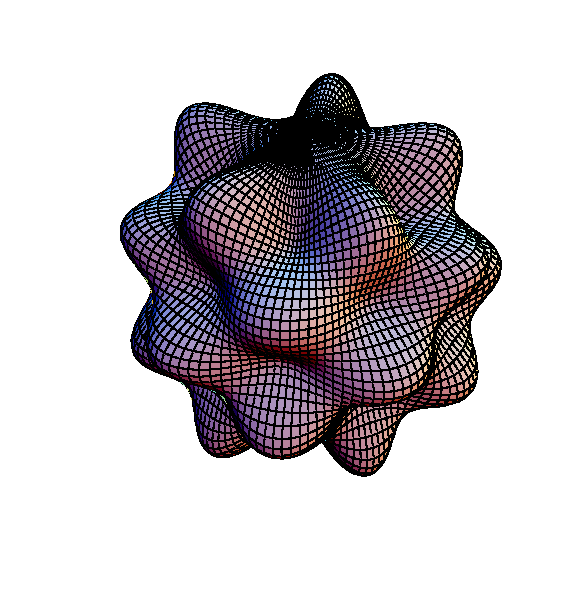
\includegraphics[width=0.3\textwidth]{sh_r_9_5}
  \end{figure}
\end{frame}

\begin{frame}
  \frametitle{Outline}
  \tableofcontents[pausesections]
  % You might wish to add the option [pausesections]
\end{frame}


% Structuring a talk is a difficult task and the following structure
% may not be suitable. Here are some rules that apply for this
% solution: 

% - Exactly two or three sections (other than the summary).
% - At *most* three subsections per section.
% - Talk about 30s to 2min per frame. So there should be between about
%   15 and 30 frames, all told.

% - A conference audience is likely to know very little of what you
%   are going to talk about. So *simplify*!
% - In a 20min talk, getting the main ideas across is hard
%   enough. Leave out details, even if it means being less precise than
%   you think necessary.
% - If you omit details that are vital to the proof/implementation,
%   just say so once. Everybody will be happy with that.

\section{Fourier Analysis on \twosphere}

\subsection{$\mathbb{S}^1$: Complex Exponentials $e^{\im k \vphi}$}

\begin{frame}
  \frametitle{$\mathbb{S}^1$: Complex Exponentials $e^{\im k \vphi}$}
  
  \begin{center}
  
%  \begin{minipage}[t]{0.5\textwidth}
	  \begin{tabular}{c}
%	    Approximation space \\  
%	    $\Ln{2}{\R^2}$\\
%	    \pause
%	    \textarrowup{dense in} \\
	    Polynomials in $\R^2$\\
	    $\fun{\Pi}{\R^2}$ \\
	    \pause
	    \textarrowdown{restrict to} \\
	    Homogeneous polynomials in $\R^2$\\
	    $\fun{\text{Hom}}{\R^2} := \pset{f \in \fun{\Pi_{k}}{\R^2}}{|}{k \in \NZ,\ \fun{f}{\lambda\V{x}} = \lambda^k \fun{f}{\V{x}}}$ \\
	    \pause
	    \textarrowdown{restrict to} \\
	    Homogeneous harmonic polynomials in $\R^2$ \\ 
	    $\fun{\text{Harm}}{\R^2} := \pset{f \in \fun{\Pi_{k}}{\R^2}}{|}{k \in \NZ,\ \fun{f}{\lambda\V{x}} = \lambda^k \fun{f}{\V{x}},\ \Delta_{\V{x}} f \equiv 0}$
	  \end{tabular}
%	\end{minipage}
%	\hfill
%  \begin{minipage}[b]{0.3\textwidth}
%    \begin{pgfpicture}{0cm}{0cm}{2cm}{3cm} 
%      \only<6->
%      {
%	      \pgfnodecircle{Node1}[stroke]{\pgfxy(-7,-2.6)}{0.0cm} 
%	      \pgfnodecircle{Node2}[stroke]{\pgfxy(-3.8,2.8)}{0.0cm}     
%	      \pgfsetlinewidth{1.0pt}
%	      \color{structure}
%	      \pgfsetendarrow{\pgfarrowto}
%	      \pgfnodeconncurve{Node1}{Node2}{110}{200}{3cm}{3cm}
%	    }
%      \only<5>{\pgfputat{\pgfxy(-6.2,2.0)}{\pgfbox[right,center]{\alert{{Surprise}}}}}
%      \only<6->{\pgfputat{\pgfxy(-6.2,2.0)}{\pgfbox[right,center]{dense in}}}
%    \end{pgfpicture}
%	\end{minipage}

  \end{center}

\end{frame}

\begin{frame}
  \frametitle{$\mathbb{S}^1$: Complex Exponentials $e^{\im k \vphi}$}
  
  \begin{itemize}
    \item Homogeneous polynomials separate in polar coordinates:\\
          $p_{k} \in \fun{\text{Hom}}{\R^2}, \deg p_{k} = k, k \in \NZ$
          \[\Rightarrow \fun{p_{k}}{r,\vphi} = r^k \fun{q_{k}}{\vphi}\ \paren{r \in \Rp,\ 
          \vphi \in \interv{[}{0}{2\pi}{)}}\]
    \pause  
    \item Laplacian in Cartesian coordinates:
      \[\Delta_{\V{x}} = \frac{\partial^2}{\partial x_{1}^2} + \frac{\partial^2}{\partial x_{2}^2}\]
     \pause
    \item Laplacian in polar coordinates:
      \[\Delta_{\paren{r,\vphi}} = \frac{1}{r^2} \frac{\partial^2}{\partial \vphi^2} +  \frac{\partial^2}{\partial r^2} + \frac{1}{r}\frac{\partial}{\partial r}\]
  \end{itemize}

\end{frame}

\begin{frame}
  \frametitle{$\mathbb{S}^1$: Complex Exponentials $e^{\im k \vphi}$}

  \vspace{-1.0cm}
  \begin{itemize}
    \item A homogeneous harmonic polynomial $\fun{p_{k}}{r,\vphi} = r^k \fun{q_{k}}{\vphi}$ fulfills
      \[
        r^{k-2} \paren{k^2 \fun{q_{k}}{\vphi} + \fun{q_{k}''}{\vphi}} = 0
      \]
    \uncover<2->
    {  
      \item Equivalently, if $r=1$, $q_{k}$ is an eigenfunction of the \emph{Circular Laplacian}
    }
    \end{itemize}  
    \uncover<2->
    {
      \[\Delta_{\vphi} = \frac{\partial^2}{\partial \vphi^2}\]
    }
  \begin{columns}
    \column{4cm}
    \column{4cm}
    \uncover<3->
    {
		  \begin{block}{Eigenfunctions}
		  \[
		     \e^{\im k \varphi} \quad \paren{k \in \Z}
		  \]
		  \end{block}
		}
    \column{4cm}
	    \begin{pgfpicture}{0cm}{0cm}{1cm}{1cm} 
	      \only<3->
	      {
		      \pgfnodecircle{Node1}[stroke]{\pgfxy(-1,2.2)}{0.0cm} 
		      \pgfnodecircle{Node2}[stroke]{\pgfxy(0.3,1.1)}{0.0cm}     
		      \pgfsetlinewidth{1.0pt}
		      \color{structure}
		      \pgfsetendarrow{\pgfarrowto}
		      \pgfnodeconncurve{Node1}{Node2}{0}{40}{1.5cm}{1.5cm}
		    }
		    \color{black}
%	      \only<4->
%	      {
%		      \pgfnodecircle{Node1}[stroke]{\pgfxy(-6,-1.0)}{0.0cm} 
%		      \pgfnodecircle{Node2}[stroke]{\pgfxy(-4.6,0.3)}{0.0cm}     
%		      \pgfsetlinewidth{1.0pt}
%		      \color{structure}
%		      \pgfsetendarrow{\pgfarrowto}
%		      \pgfnodeconncurve{Node1}{Node2}{90}{-180}{1.0cm}{1.0cm}
%	        \pgfputat{\pgfxy(-6,-2.0)}{\pgfbox[center,center]
%	        {\parbox{3cm}{\begin{center}homogeneous \\ harmonic \\ polynomials in $\R^2$\end{center}}}}
%		    }
	      \only<4->
	      {
%		      \pgfnodecircle{Node1}[stroke]{\pgfxy(-2.2,-1.1)}{0.0cm} 
%		      \pgfnodecircle{Node2}[stroke]{\pgfxy(-2.2,-0.6)}{0.0cm}     
%		      \pgfsetlinewidth{1.0pt}
%		      \color{structure}
%		      \pgfsetendarrow{\pgfarrowto}
%		      \pgfnodeconncurve{Node1}{Node2}{90}{-90}{1.0cm}{1.0cm}
	        \pgfputat{\pgfxy(-2.2,-1.0)}{\pgfbox[center,center] 
	        {\parbox{10cm}{\begin{center}form a complete orthogonal system in $\Ln{2}{\mathbb{S}^1}$\end{center}}}}	
	      }
%	      \only<5->
%	      {
%		      \pgfnodecircle{Node1}[stroke]{\pgfxy(1.6,-1.0)}{0.0cm} 
%		      \pgfnodecircle{Node2}[stroke]{\pgfxy(0.2,0.3)}{0.0cm}     
%		      \pgfsetlinewidth{1.0pt}
%		      \color{structure}
%		      \pgfsetendarrow{\pgfarrowto}
%		      \pgfnodeconncurve{Node1}{Node2}{90}{0}{1.0cm}{1.0cm}
%	        \pgfputat{\pgfxy(1.6,-2.0)}{\pgfbox[center,center]
%	        {\parbox{3cm}{\begin{center} span $\left.\fun{\Pi}{\R^2}\right|_{\mathbb{S}^1}$\end{center}}}}
%	      }
	      
	      %\only<6->{\pgfputat{\pgfxy(-6.2,2.0)}{\pgfbox[right,center]{dense in}}}
	    \end{pgfpicture}
  \end{columns}  
%    \item The functions $\e^{ik\varphi}$ are homogeneous harmonic polynomials in $\R^2$ restricted to the unit circle $\mathbb{S}^1$
%    \item The functions $\e^{ik\varphi}$ are orthogonal with respect to the $\Ln{2}{\mathbb{S}^1}$ inner product
%    \item $\text{span} \pset{\e^{ik\varphi}}{|}{k \in \Z} = \left.\fun{\Pi}{\R^2}\right|_{\mathbb{S}^1}$
%  \end{itemize}
  
\end{frame}

\begin{frame}
  \frametitle{Spherical Coordinates}

  \begin{itemize}
  \item
    $\V{x} \in \R^3 \setminus \set{\V{0}}$
  \item
    $\V{x} = \paren{x_1,x_2,x_3}^{\transp} = \paren{r \sin \vtheta \cos \vphi, r \sin \vtheta \sin \vphi, r \cos \vtheta}^{\transp}$,\\ $r \in \Rp$, $\vtheta \in \interv{[}{0}{\pi}{]}$, $\vphi \in \interv{[}{0}{2\pi}{)}$
  \end{itemize}

  \begin{figure}[h]
    \centering
    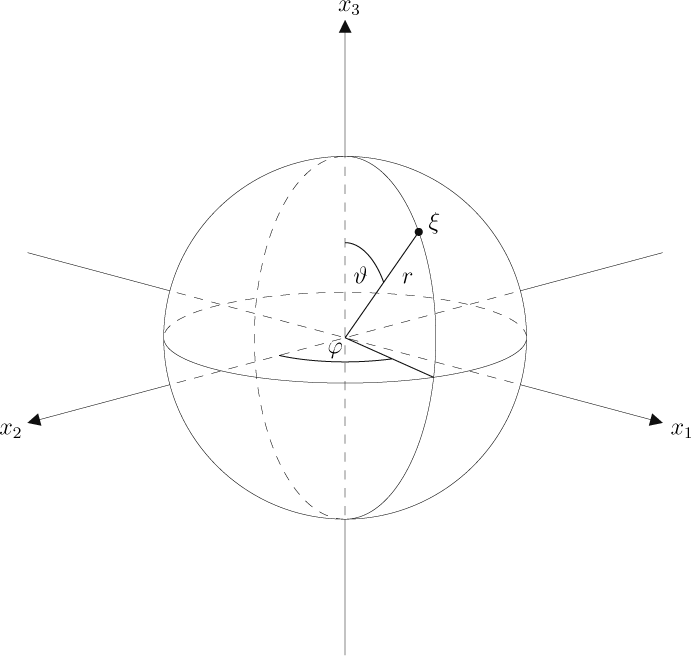
\includegraphics[width=0.5\textwidth]{sphere}
  \end{figure}

\end{frame}

\subsection{$\mathbb{S}^2$: Spherical Harmonics $Y_k^n$}

\begin{frame}
  \frametitle{$\mathbb{S}^2$: Spherical Harmonics $Y_k^n$}
  
  \begin{center}
  
%  \begin{minipage}[t]{0.5\textwidth}
	  \begin{tabular}{c}
%	    Approximation space \\  
%	    $\Ln{2}{\alert{\R^3}}$\\
%	    \pause
%	    \textarrowup{dense in} \\
	    Polynomials in $\alert{\R^3}$\\
	    $\fun{\Pi}{\alert{\R^3}}$ \\
	    \pause
	    \textarrowdown{restrict to} \\
	    Homogeneous polynomials in $\alert{\R^3}$\\
	    $\fun{\text{Hom}}{\alert{\R^3}} := \pset{f \in \fun{\Pi_{k}}{\alert{\R^3}}}{|}{k \in \NZ,\ \fun{f}{\lambda\V{x}} = \lambda^k \fun{f}{\V{x}}}$ \\
	    \pause
	    \textarrowdown{restrict to} \\
	    Homogeneous harmonic polynomials in $\alert{\R^3}$ \\ 
	    $\fun{\text{Harm}}{\alert{\R^3}} := \pset{f \in \fun{\Pi_{k}}{\alert{\R^3}}}{|}{k \in \NZ,\ \fun{f}{\lambda\V{x}} = \lambda^k \fun{f}{\V{x}},\ \Delta_{\V{x}} f \equiv 0}$
	  \end{tabular}
%	\end{minipage}
%	\hfill
%  \begin{minipage}[b]{0.3\textwidth}
%    \begin{pgfpicture}{0cm}{0cm}{2cm}{3cm} 
%      \only<6->
%      {
%	      \pgfnodecircle{Node1}[stroke]{\pgfxy(-7,-2.6)}{0.0cm} 
%	      \pgfnodecircle{Node2}[stroke]{\pgfxy(-3.8,2.8)}{0.0cm}     
%	      \pgfsetlinewidth{1.0pt}
%	      \color{structure}
%	      \pgfsetendarrow{\pgfarrowto}
%	      \pgfnodeconncurve{Node1}{Node2}{110}{200}{3cm}{3cm}
%	    }
%      \only<5>{\pgfputat{\pgfxy(-6.2,2.0)}{\pgfbox[right,center]{\alert{{Big surprise}}}}}
%      \only<6->{\pgfputat{\pgfxy(-6.2,2.0)}{\pgfbox[right,center]{dense in}}}
%    \end{pgfpicture}
%	\end{minipage}

  \end{center}

\end{frame}

\begin{frame}
  \frametitle{$\mathbb{S}^2$: Spherical Harmonics $Y_k^n$}
  
  \begin{itemize}
    \item Homogeneous polynomials separate in \alert{spherical} coordinates:\\
          $p_{k} \in \fun{\text{Hom}}{\alert{\R^3}}, \deg p_{k} = k, k \in \NZ$
          \[\Rightarrow \fun{p_{k}}{r,\alert{\vtheta,}\vphi} = r^k
          \fun{q_{k}}{\alert{\vtheta,}\vphi}\ \paren{r \in \Rp,\ 
          \alert{\vtheta \in \interv{[}{0}{\pi}{]},} \
          \vphi \in \interv{[}{0}{2\pi}{)}}\]
    \pause  
    \item Laplacian in Cartesian coordinates:
      \[\Delta_{\V{x}} = \frac{\partial^2}{\partial x_{1}^2} + 
      \frac{\partial^2}{\partial x_{2}^2} + 
      \alert{\frac{\partial^2}{\partial x_{3}^2}}\]
     \pause
    \item Laplacian in \alert{spherical} coordinates:
      \[\Delta_{\paren{r,\vtheta,\vphi}} = \frac{1}{r^2 \alert{\sin^2 \vtheta}} \frac{\partial^2}{\partial \vphi^2} +  \frac{\partial^2}{\partial r^2} + \frac{\alert{2}}{r}\frac{\partial}{\partial r} + \alert{\frac{1}{r^2 \sin \vtheta}�\frac{\partial}{\partial \vtheta} \paren{\sin \vtheta \: \frac{\partial}{\partial \vtheta}}}\]
  \end{itemize}

\end{frame}

\begin{frame}
  \frametitle{$\mathbb{S}^2$: Spherical Harmonics $Y_k^n$}

  \vspace{-1.0cm}
    \begin{itemize}
    \item If $r = 1$, a homogeneous harmonic polynomial $\fun{p_{k}}{r,\vtheta,\vphi} =
      \fun{q_{k}}{\vtheta,\vphi}$ fulfills
      \[
        \Delta_{\paren{\vtheta,\vphi}} \fun{q_{k}}{\vtheta,\vphi} = -k(k-1) \fun{q_{k}}{\vtheta,\vphi}
      \]
      with the \emph{Spherical Laplacian}
    \end{itemize}  
    \[
     \Delta_{\paren{\vtheta,\vphi}} = \frac{1}{\alert{\sin^2 \vtheta}} 
     \frac{\partial^2}{\partial \vphi^2} + \alert{\frac{1}{ \sin \vtheta}�
     \frac{\partial}{\partial \vtheta} \paren{\sin \vtheta \: \frac{\partial}{\partial \vtheta}}}
    \]
  \begin{columns}
    \column{0.1cm}
    \column{11cm}
    \uncover<2->
    {
		  \begin{block}{Eigenfunctions}
		  \vspace{-1ex}
		  \[
%        \alert
%        {
          \fun{Y_{k}^n}{\vtheta,\vphi} := \sqrt{\frac{2k+1}{4\pi}}
          \fun{P_{k}^{\abs{n}}}{\cos \vtheta} \e^{i n \varphi} \quad 
          \paren{k \in \NZ,\ n = -k,\ldots,k}
%        }
		  \]
		  \end{block}
		}
    \column{0.1cm}
	    \begin{pgfpicture}{0cm}{0cm}{1cm}{1cm} 
	      \only<2->
	      {
		      \pgfnodecircle{Node1}[stroke]{\pgfxy(-2.2,2.6)}{0.0cm} 
		      \pgfnodecircle{Node2}[stroke]{\pgfxy(-1.4,1.7)}{0.0cm}     
		      \pgfsetlinewidth{1.0pt}
		      \color{structure}
		      \pgfsetendarrow{\pgfarrowto}
		      \pgfnodeconncurve{Node1}{Node2}{0}{90}{0.7cm}{0.7cm}
		    }
		    \color{black}
%	      \only<3->
%	      {
%		      \pgfnodecircle{Node1}[stroke]{\pgfxy(-9.8,-1.6)}{0.0cm} 
%		      \pgfnodecircle{Node2}[stroke]{\pgfxy(-9.8,-1.0)}{0.0cm}     
%		      \pgfsetlinewidth{1.0pt}
%		      \color{structure}
%		      \pgfsetendarrow{\pgfarrowto}
%		      \pgfnodeconncurve{Node1}{Node2}{90}{-90}{1.0cm}{1.0cm}
%	        \pgfputat{\pgfxy(-9.8,-2.4)}{\pgfbox[center,center]
%	        {\parbox{3cm}{\begin{center}homogeneous \\ harmonic \\ polynomials in $\alert{\R^2}$\end{center}}}}
%		    }
	      \only<3->
	      {
%		      \pgfnodecircle{Node1}[stroke]{\pgfxy(-5.8,-1.6)}{0.0cm} 
%		      \pgfnodecircle{Node2}[stroke]{\pgfxy(-5.8,-1.0)}{0.0cm}     
%		      \pgfsetlinewidth{1.0pt}
%		      \color{structure}
%		      \pgfsetendarrow{\pgfarrowto}
%		      \pgfnodeconncurve{Node1}{Node2}{90}{-90}{1.0cm}{1.0cm}
	        \pgfputat{\pgfxy(-5.8,-1.4)}{\pgfbox[center,center] 
	        {\parbox{10cm}{\begin{center}form a complete orthonormal system in 
	          $\Ln{2}{\alert{\mathbb{S}^2}}$\end{center}}}}	
	      }
%	      \only<5->
%	      {
%		      \pgfnodecircle{Node1}[stroke]{\pgfxy(-1.8,-1.6)}{0.0cm} 
%		      \pgfnodecircle{Node2}[stroke]{\pgfxy(-1.8,-1.0)}{0.0cm}     
%		      \pgfsetlinewidth{1.0pt}
%		      \color{structure}
%		      \pgfsetendarrow{\pgfarrowto}
%		      \pgfnodeconncurve{Node1}{Node2}{90}{-90}{1.0cm}{1.0cm}
%	        \pgfputat{\pgfxy(-1.8,-2.4)}{\pgfbox[center,center]
%	        {\parbox{3cm}{\begin{center} span $\left.\fun{\Pi}{\alert{\R^3}}\right|_{\alert{\mathbb{S}^2}}$\end{center}}}}
%	      }
	    \end{pgfpicture}
  \end{columns}  
  
\end{frame}

\begin{frame}
  \frametitle{$\mathbb{S}^2$: Spherical Harmonics $Y_k^n$}
  \begin{figure}[h]
    \centering
    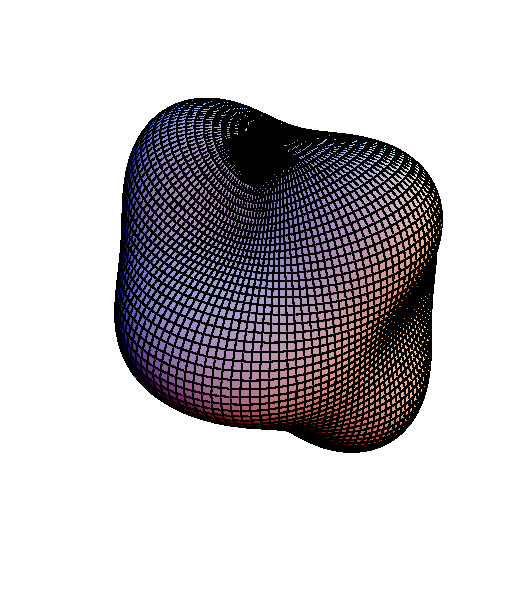
\includegraphics[width=0.5\textwidth]{sh_r_4_2}\\
    $\Re \: Y_{4}^{2}$
  \end{figure} 
\end{frame}  

\begin{frame}
  \frametitle{$\mathbb{S}^2$: Spherical Harmonics $Y_k^n$}
  \begin{figure}[h]
    \centering
    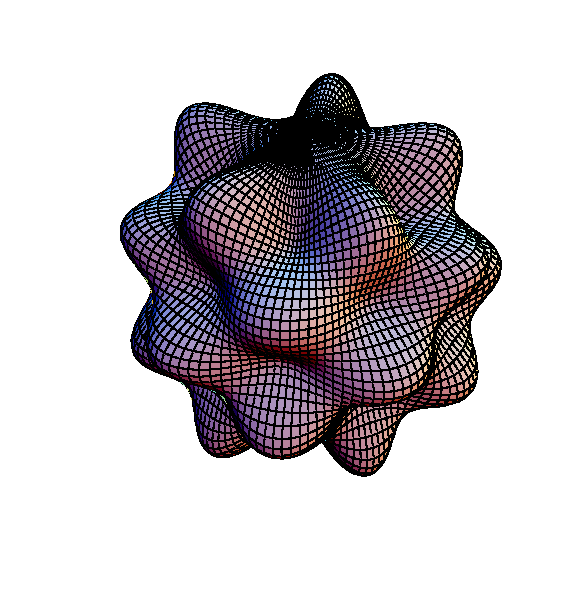
\includegraphics[width=0.5\textwidth]{sh_r_9_5}\\
    $\Re \: Y_{9}^{5}$
  \end{figure}
\end{frame}  

\begin{frame}
  \frametitle{$\mathbb{S}^2$: Spherical Harmonics $Y_k^n$}
  \begin{figure}[h]
    \centering
    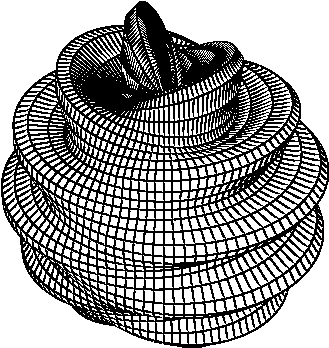
\includegraphics[width=0.5\textwidth]{sh_r_13_1}\\
    $\Re \: Y_{13}^{1}$
  \end{figure}
\end{frame}  

\begin{frame}
  \frametitle{$\mathbb{S}^2$: Spherical Harmonics $Y_k^n$}
  \begin{figure}[h]
    \centering
    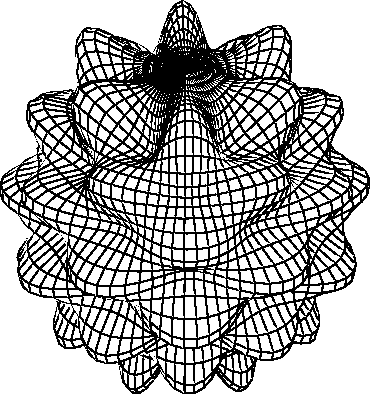
\includegraphics[width=0.5\textwidth]{sh_r_13_6}\\
    $\Re \: Y_{13}^{6}$
  \end{figure}
\end{frame}  

\begin{frame}
  \frametitle{$\mathbb{S}^2$: Spherical Harmonics $Y_k^n$}
  \begin{figure}[h]
    \centering
    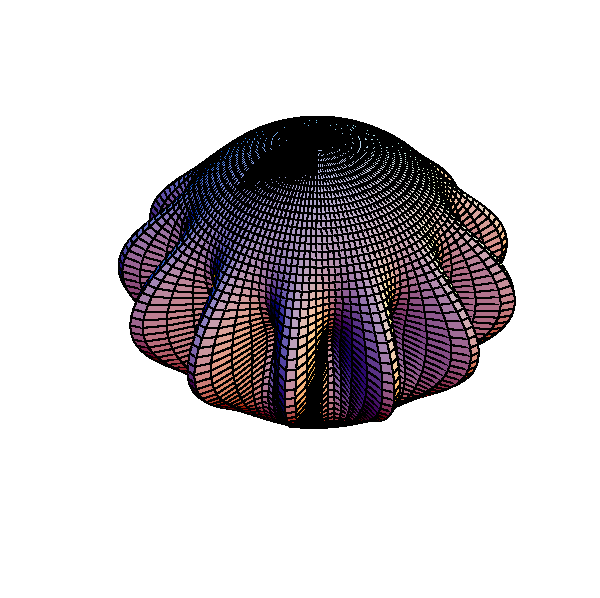
\includegraphics[width=0.5\textwidth]{sh_r_13_13}\\
    $\Re \: Y_{13}^{13}$
  \end{figure}
\end{frame}  

%    \item Eigenfunctions: 
%      \[
%      \]  
%    \item The functions $\e^{ik\varphi}$ are homogeneous harmonic polynomials in 
%      $\R^2$ restricted to the unit circle $\mathbb{S}^1$
%    \item The functions $\e^{ik\varphi}$ are orthogonal with respect to 
%      the $\Ln{2}{\mathbb{S}^1}$ inner product
%    \item $\text{span} \pset{\e^{ik\varphi}}{|}{k \in \Z} = \left.\fun{\Pi}{\R^3}\right|_{\mathbb{S}^1}$

%\begin{frame}
%  \frametitle{Comparison $\mathbb{S}^1$ and $\twosphere$}

%  \newcolumntype{C}{>{$}c<{$}} 
%  \newcolumntype{L}{>{$}l<{$}} 
%  \newcolumntype{R}{>{$}r<{$}} 
%  \setlength{\extrarowheight}{5pt}

%  {\tiny
%  \begin{tabular}{|l|C|C|}
%    \firsthline
%               & \mathbb{S}^1 & \twosphere \\[5pt] \hline
%    Definition & \mathbb{S}^1 := \mathbb{T}^1 := \pset{\V{x} \in \R^2}{|}{\norm{\V{x}}_{2} = 1} &
%    \twosphere := \pset{\V{x} \in \R^{3}}{|}{\norm{\V{x}}_2 = 1} \\[5pt] \hline
%    Laplace's equation & \frac{\partial^2}{\partial x_1^2} + \frac{\partial^2}{\partial x_2^2} = 0 &
%    \frac{\partial^2}{\partial x_1^2} + \frac{\partial^2}{\partial x_2^2} + \frac{\partial^2}{\partial x_3^2} = 0 \\[5pt] \lasthline
%  \end{tabular}
%  }
%  
%  You can create overlays\dots
%  \begin{itemize}
%  \item using the \texttt{pause} command:
%    \begin{itemize}
%    \item
%      First item.
%      \pause
%    \item    
%      Second item.
%    \end{itemize}
%  \item
%    using overlay specifications:
%    \begin{itemize}
%    \item<3->
%      First item.
%    \item<4->
%      Second item.
%    \end{itemize}
%  \item
%    using the general \texttt{uncover} command:
%    \begin{itemize}
%      \uncover<5->{\item
%        First item.}
%      \uncover<6->{\item
%        Second item.}
%    \end{itemize}
%  \end{itemize}
%\end{frame}

\section{Nonequispaced Fast Spherical Fourier Transform (NFSFT)}

\subsection{Introduction}

\begin{frame}
  \frametitle{Some notation}
  
  \begin{itemize}
    \item Bandwidth: $M \in \NZ$, $t := \ceil{\log_{2}M}$, $N := 2^t$
    \pause
    \item Sampling set: $\mathcal{X} := \paren{\vtheta_d,\vphi_d}_{d=0}^{D-1} \quad \paren{D \in \N}$
    \pause
    \item Index set: $\mathcal{I}^M := \pset{\paren{k,n}}{|}{k=0,\ldots,M;n=-k,\ldots,k}$
    \pause
    \item Fourier expansion of $f: \twosphere \rightarrow \C$ with bandwidth $M \in \NZ$: 
      \[ f = \sum_{\paren{k,n} \in \mathcal{I}^M} \fun{a_k^n}{f} Y_{k}^n,\]
    \pause
    \item Spherical Fourier coefficients: $a_{k}^n = \fun{a_k^n}{f}$
  \end{itemize}
\end{frame}

\begin{frame}
  \frametitle{Nonequispaced Discrete Spherical Fourier Transform}
  \begin{block}{Nonequispaced Discrete Spherical Fourier Transform (NDSFT)}
    Given Fourier coefficients $a_k^n$ for $\paren{k,n} \in \mathcal{I}^M$ and a 
    sampling set $\mathcal{X}$, evaluate
    \[
      \fun{f}{\vtheta_d,\vphi_d} = \sum_{\paren{k,n} \in \mathcal{I}^M}
      a_k^n \fun{Y_{k}^n}{\vtheta_d,\vphi_d} 
      \quad \paren{\paren{\vtheta_d,\vphi_d} \in \mathcal{X}}.
    \]
  \end{block}
  
  \begin{center}
    \alert
    {
      \begin{align}
        \pause
        \nonumber \text{Naivest algorithm} & \longrightarrow \bigo{M^3 D}\ \text{flops} \\
        \pause
        \nonumber \text{``Direct'' algorithm} & \longrightarrow \bigo{M^2 D}\ \text{flops}
      \end{align}
    }
  \end{center}
\end{frame}

\begin{frame}
  \frametitle{Nonequispaced Fast Spherical Fourier Transform}
  
  %\vspace{-0.5cm}
  %\hspace{-4ex}(Kunis, Potts, Steidl, Tasche)
  \begin{center}
    \vspace{-0.5cm}
	  \begin{tabular}{c}
	    \parbox[b]{10cm}
	    {
	      \begin{center}
	          $\displaystyle \fun{f}{\vtheta,\vphi} = 
	             \displaystyle 
	             \only<1>{\sum_{\paren{k,n} \in \mathcal{I}^M} a_k^n \fun{Y_{k}^n}{\vtheta,\vphi}}
	             \only<2>{\sum_{k = 0}^M \sum_{n = -k}^k a_k^n \fun{Y_{k}^n}{\vtheta,\vphi}}
	             \only<3>{\sum_{n = -M}^M \sum_{k = \abs{n}}^M a_k^n \fun{Y_{k}^n}{\vtheta,\vphi}}
	             \only<4->{\sum_{n = -M}^M \paren{\sum_{k = \abs{n}}^M a_k^n \fun{P_{k}^{\abs{n}}}{\cos \vtheta}} \e^{\im n \vphi}}
	            $ 
	      \end{center}
	    } \\
	    \visible<5-10>
	    {
	      \begin{pgfpicture}{0cm}{0cm}{4cm}{0.5cm} 
          \pgfnodecircle{Node1}[stroke]{\pgfxy(2.8,0.7)}{0.0cm} 
	        \pgfnodecircle{Node2}[stroke]{\pgfxy(-0.4,-0.5)}{0.0cm}     
          \pgfnodecircle{Node3}[stroke]{\pgfxy(2.8,0.7)}{0.0cm} 
	        \pgfnodecircle{Node4}[stroke]{\pgfxy(4.6,-0.5)}{0.0cm}     
		      \pgfsetlinewidth{1.0pt}
		      \color{structure}
		      \pgfsetendarrow{\pgfarrowto}
		      \pgfnodeconncurve{Node1}{Node2}{-90}{90}{1.0cm}{1.0cm}
		      \pgfnodeconncurve{Node3}{Node4}{-90}{90}{1.0cm}{1.0cm}
	        \pgfputat{\pgfxy(-1.0,0.0)}{\pgfbox[center,center]{$n$ even}}
	        \pgfputat{\pgfxy(5.2,-0.0)}{\pgfbox[center,center]{$n$ odd}}
        \end{pgfpicture}\\
   	    \parbox[b][2cm][c]{5cm}
	      {
	        \begin{center}
	            $\displaystyle 
	              \only<-5>{\uncover<5>{\sum_{k = \abs{n}}^M a_k^n \fun{P_{k}^{\abs{n}}}{\cos \vtheta}}}
	              \only<6>{\sum_{k = 0}^M b_k^n \fun{T_{k}}{\cos \vtheta}}
	              \only<7>{\sum_{k = 0}^M b_k^n \fun{\cos}{k \vtheta}}
	              \only<8->{\sum_{k = -M}^M c_k^n \e^{\im k \vtheta}}
	            $ 
  	        \end{center}
	      }
   	    \parbox[b][2cm][c]{5cm}
	      {
	        \begin{center}
	            $\displaystyle 
	              \only<-5>{\uncover<5>{\sum_{k = \abs{n}}^M a_k^n \fun{P_{k}^{\abs{n}}}{\cos \vtheta}}}
	              \only<6>{\sin{\vtheta} \sum_{k = 0}^{M-1} b_k^n \fun{T_{k}}{\cos \vtheta}}
	              \only<7>{\sin{\vtheta} \sum_{k = 0}^{M-1} b_k^n \fun{\cos}{k \vtheta}}
	              \only<8->{\sum_{k = -M}^{M} c_k^n \e^{\im k \vtheta}}
	            $ 
  	        \end{center}
	      }
	    }\\
	    \visible<9->
	    {
	      \begin{pgfpicture}{0cm}{0cm}{4cm}{0.5cm} 
          \pgfnodecircle{Node1}[stroke]{\pgfxy(-0.4,0.7)}{0.0cm} 
	        \pgfnodecircle{Node2}[stroke]{\pgfxy(3.4,-0.3)}{0.0cm}     
          \pgfnodecircle{Node3}[stroke]{\pgfxy(4.6,0.7)}{0.0cm} 
	        \pgfnodecircle{Node4}[stroke]{\pgfxy(3.4,-0.3)}{0.0cm}     
		      \pgfsetlinewidth{1.0pt}
		      \color{structure}
		      \pgfsetendarrow{\pgfarrowto}
		      \pgfnodeconncurve{Node1}{Node2}{-90}{90}{1.0cm}{1.0cm}
		      \pgfnodeconncurve{Node3}{Node4}{-90}{90}{1.0cm}{1.0cm}
        \end{pgfpicture}\\
	      $\displaystyle \fun{f}{\vtheta,\vphi} = \sum_{n = -M}^M \sum_{k = -M}^M c_k^n 
	      \e^{\im k \vtheta} \e^{\im n \vphi}$
	    }
    \end{tabular}
  \end{center}
  
\end{frame}

\begin{frame}
  \frametitle{Nonequispaced Fast Spherical Fourier Transform}

  \begin{columns}
  
    \column{5cm}
    
	      \begin{pgfpicture}{-0.6cm}{-0.6cm}{5cm}{5cm} 
          \pgfsetlinewidth{1.0pt}
          \visible<1>
          {
	          \begin{pgfscope}
	            \pgfmoveto{\pgfxy(3.00,2.00)} 
	            \pgflineto{\pgfxy(5.00,0.00)} 
	            \pgflineto{\pgfxy(5.00,4.00)} 
	            \pgfclip 
	            \color{MyBlue}
	            \pgfrect[fill]{\pgfxy(3.00,0.00)}{\pgfxy(5.00,4.00)} 
	          \end{pgfscope}
	        }
          \visible<2>
          {
	          \begin{pgfscope}
	            \pgfmoveto{\pgfxy(3.00,0.00)} 
	            \pgflineto{\pgfxy(5.00,0.00)} 
	            \pgflineto{\pgfxy(5.00,4.00)} 
	            \pgflineto{\pgfxy(3.00,4.00)} 
	            \pgfclip 
	            \color{MyGreen}
	            \pgfrect[fill]{\pgfxy(3.00,0.00)}{\pgfxy(5.00,4.00)} 
	          \end{pgfscope}
	        }
          \visible<3->
          {
	          \begin{pgfscope}
	            \pgfmoveto{\pgfxy(1.00,0.00)} 
	            \pgflineto{\pgfxy(5.00,0.00)} 
	            \pgflineto{\pgfxy(5.00,4.00)} 
	            \pgflineto{\pgfxy(1.00,4.00)} 
	            \pgfclip 
	            \color{MyRed}
	            \pgfrect[fill]{\pgfxy(1.00,0.00)}{\pgfxy(5.00,4.00)} 
	          \end{pgfscope}
	        }
          \color{structure}
          \faxes{0.00}{-1.00}{6.00}{5.00}{0.2}{0.2}{$k$}{$n$}
%          \pgfsetendarrow{\pgfarrowto}
%          \pgfline{\pgfxy(0,2)}{\pgfxy(6,2)} 
%          \pgfline{\pgfxy(3,-1)}{\pgfxy(3,5)} 
%	        \pgfputat{\pgfxy(6.2,2.0)}{\pgfbox[left,center]{$k$}}
%	        \pgfputat{\pgfxy(3.0,5.2)}{\pgfbox[center,bottom]{$n$}}
          \color{black}
          \visible<1>
          {
            \ftriangle{3.00}{2.00}{0.25}{0.25}{9}{0.05cm}
          }  
          \visible<2>
          {
            \frect{3.00}{0.00}{0.25}{0.25}{9}{17}{0.05cm}
          }
          \visible<3->
          {
            \frect{1.00}{0.00}{0.25}{0.25}{17}{17}{0.05cm}
          }
	      \end{pgfpicture}
    \column{7.7cm}
      \vspace{-3ex}
			  \begin{tabular}{c}
			    $\color{MyBlue}\paren{a_{k}^n}$ \\
			    \pause
			    \textarrowdown{FLFT $\bigo{M^2 \log^2 M}$} \\
			    $\color{MyGreen}\paren{b_{k}^n}$ \\
			    \pause
			    \textarrowdown{"magic" $\bigo{M^2}$} \\
			    $\color{MyRed}\paren{c_{k}^n}$ \\
			    \pause
			    \textarrowdown{2D-NFFT \tiny $\bigo{M^2 \log M + \log\frac{1}{\varepsilon}D}$} \\
			    $\paren{\fun{f}{\vtheta_{d},\vphi_{d}}}_{d=0}^{D-1}$ \\
			  \end{tabular}	  
  \end{columns}
  
\end{frame}

\subsection{Fast Legendre Function Transform}

\begin{frame}
  \frametitle{Associated Legendre Functions}
  \begin{block}{Definition: Associated Legendre Functions}
    \begin{itemize}
      \item $P_{k}^n: \interv{[}{-1}{1}{]} \rightarrow \R \ \paren{k,n \in \NZ, n \le k}$
      \item $P_{k}^n := \paren{\frac{(k-n)!}{(k+n)!}}^{1/2} \paren{1-x^2}^{n/2} \frac{\dx^n}{\dx x^n} P_{k}$
    \end{itemize}
  \end{block}  

  \parbox[t][3cm]{10cm}
  {
  \only<-2>
  {
    \uncover<2>
    {
		  \begin{block}{Three-term Recurrence}
		    \begin{itemize}
		      \item $\fun{P_{n-1}^n}{x} := 0$
		      \item $\fun{P_{n}^n}{x} := \frac{\sqrt{(2n)!}}{2^nn!}\paren{1-x^2}^{n/2}$
		      \item $\fun{P_{k+1}^n}{x} = v_{k}^n x \fun{P_{k}^n}{x} + w_{k}^n \fun{P_{k-1}^n}{x} \ \paren{k,n \in \NZ,\ k \ge n}$
		    \end{itemize}
		  \end{block}
		}
  }
  \only<3>
  {
		  \begin{block}{\alert{Extended} Three-term Recurrence (Potts, Steidl, Tasche)}
		    \begin{itemize}
		      \item n even: $\fun{P_{-1}^n}{x} := 0,\ \fun{P_{0}^n}{x} := \frac{\sqrt{(2n)!}}{2^nn!}$
		      \item n odd: $\fun{P_{0}^n}{x} := \fun{P_{1}^n}{x} := \frac{\sqrt{(2n)!}}{2^nn!}\left(1-x^2\right)^{1/2}$
		      \item $\fun{P_{k+1}^n}{x} = \paren{\alpha_{k}^n x + \beta_{k}^n}\fun{P_{k}^n}{x} + \gamma_{k}^n \fun{P_{k-1}^n}{x}$
		    \end{itemize}
		  \end{block}
  }
  }
\end{frame}

\begin{frame}
  \frametitle{Associated Legendre Functions}
  
  \begin{block}{Definition: Associated Legendre Polynomials}
    \begin{itemize}
      \item $\fun{P_{-1}^n}{x,c}  := 0$,\\
      \item $\fun{P_{0}^n}{x,c}   := 1$,\\
      \item $\fun{P_{k+1}^n}{x,c}  = \paren{\alpha_{k+c}^n x + \beta_{k+c}^n} \fun{P_{k}^n}{x,c} + \gamma_{k+c}^n \fun{P_{k-1}^n}{x,c}.$    
    \end{itemize}  
  \end{block}  
  
  \begin{block}{Lemma}
    $\displaystyle \fun{P_{c+k}^n}{x} = \fun{P_{k}^n}{x,c}\fun{P_{c}^n}{x} + \gamma_{c}^n\fun{P_{k-1}^n}{x,c+1}\fun{P_{c-1}^n}{x}$
  \end{block}
  
  \begin{itemize}
    \item For sake of simplicity: $n \ge 0$, $n$ even
    \item Idea: $\displaystyle \sum_{k = n}^M a_{k}^n P_{k}^{n}$ \hspace{0.2cm}
      \begin{pgfpicture}{0cm}{0cm}{1.0cm}{0.2cm} 
        \pgfsetlinewidth{1.0pt}
        \color{structure}
        \pgfsetendarrow{\pgfarrowto}
        \pgfline{\pgfxy(0.0,0.0)}{\pgfxy(1.0,0.0)} 
      \end{pgfpicture}
      \hspace{0.2cm}
      $\displaystyle a_{0}^{(t-1)} P_{0}^{n} + a_{1}^{(t-1)} P_{1}^{n}$\\
      with $a_{0}^{(t-1)},\ a_{1}^{(t-1)} \in \Pi_{M}$
  \end{itemize}

\end{frame}

\begin{frame}
  \frametitle{Cascade Summation}
  
  \begin{example}
    \begin{itemize}
      \item $M = 16$, $n = 4$
    \end{itemize}
      \begin{pgfpicture}{-0.15cm}{-5.2cm}{10.70cm}{0.2cm} 
        \pgfsetlinewidth{1.0pt}
        \color{structure}
        \pgfsetendarrow{\pgfarrowtriangle{2pt}}
        \visible<2->
        {
	        \pgfputat{\pgfxy(0.00,0.0)}{\pgfbox[center,center]{$0$}}
	        \pgfputat{\pgfxy(0.65,0.0)}{\pgfbox[center,center]{$0$}}
	        \pgfputat{\pgfxy(1.30,0.0)}{\pgfbox[center,center]{$0$}}
	        \pgfputat{\pgfxy(1.95,0.0)}{\pgfbox[center,center]{$0$}}
	        \pgfputat{\pgfxy(2.60,0.0)}{\pgfbox[center,center]{$a_{4}^4$}}
	        \pgfputat{\pgfxy(3.25,0.0)}{\pgfbox[center,center]{$a_{5}^4$}}
	        \pgfputat{\pgfxy(3.90,0.0)}{\pgfbox[center,center]{$a_{6}^4$}}
	        \pgfputat{\pgfxy(4.55,0.0)}{\pgfbox[center,center]{$a_{7}^4$}}
	        \pgfputat{\pgfxy(5.20,0.0)}{\pgfbox[center,center]{$a_{8}^4$}}
	        \pgfputat{\pgfxy(5.85,0.0)}{\pgfbox[center,center]{$a_{9}^4$}}
	        \pgfputat{\pgfxy(6.50,0.0)}{\pgfbox[center,center]{$a_{10}^4$}}
	        \pgfputat{\pgfxy(7.15,0.0)}{\pgfbox[center,center]{$a_{11}^4$}}
	        \pgfputat{\pgfxy(7.80,0.0)}{\pgfbox[center,center]{$a_{12}^4$}}
	        \pgfputat{\pgfxy(8.45,0.0)}{\pgfbox[center,center]{$a_{13}^4$}}
	        \pgfputat{\pgfxy(9.10,0.0)}{\pgfbox[center,center]{$a_{14}^4$}}
	        \pgfputat{\pgfxy(9.75,0.0)}{\pgfbox[center,center]{$a_{15}^4$}}
	        \pgfputat{\pgfxy(10.4,0.0)}{\pgfbox[center,center]{$a_{16}^4$}}
	      } 

        \visible<3>
        {
          \color{red}
	        \pgfline{\pgfxy(0.00,-0.35)}{\pgfxy( 0.20,-0.65)} 
	        \pgfline{\pgfxy(0.65,-0.35)}{\pgfxy( 0.85,-0.65)} 
	        \pgfline{\pgfxy(1.30,-0.35)}{\pgfxy( 1.50,-0.65)} 
	        \pgfline{\pgfxy(1.95,-0.35)}{\pgfxy( 2.15,-0.65)} 
	        \pgfline{\pgfxy(2.60,-0.35)}{\pgfxy( 2.80,-0.65)} 
	        \pgfline{\pgfxy(3.25,-0.35)}{\pgfxy( 3.45,-0.65)} 
	        \pgfline{\pgfxy(3.90,-0.35)}{\pgfxy( 4.10,-0.65)} 
	        \pgfline{\pgfxy(4.55,-0.35)}{\pgfxy( 4.75,-0.65)} 
	        \pgfline{\pgfxy(5.20,-0.35)}{\pgfxy( 5.40,-0.65)} 
	        \pgfline{\pgfxy(5.85,-0.35)}{\pgfxy( 6.05,-0.65)} 
	        \pgfline{\pgfxy(6.50,-0.35)}{\pgfxy( 6.70,-0.65)} 
	        \pgfline{\pgfxy(7.15,-0.35)}{\pgfxy( 7.35,-0.65)} 
	        \pgfline{\pgfxy(7.80,-0.35)}{\pgfxy( 8.00,-0.65)} 
	        \pgfline{\pgfxy(8.45,-0.35)}{\pgfxy( 8.65,-0.65)} 
	        \pgfline{\pgfxy(9.10,-0.35)}{\pgfxy( 9.30,-0.65)} 
	        \pgfline{\pgfxy(9.75,-0.35)}{\pgfxy( 9.95,-0.65)}
	      } 
        \visible<4->
        {
          \color{structure}
	        \pgfline{\pgfxy(0.00,-0.35)}{\pgfxy( 0.20,-0.65)} 
	        \pgfline{\pgfxy(0.65,-0.35)}{\pgfxy( 0.85,-0.65)} 
	        \pgfline{\pgfxy(1.30,-0.35)}{\pgfxy( 1.50,-0.65)} 
	        \pgfline{\pgfxy(1.95,-0.35)}{\pgfxy( 2.15,-0.65)} 
	        \pgfline{\pgfxy(2.60,-0.35)}{\pgfxy( 2.80,-0.65)} 
	        \pgfline{\pgfxy(3.25,-0.35)}{\pgfxy( 3.45,-0.65)} 
	        \pgfline{\pgfxy(3.90,-0.35)}{\pgfxy( 4.10,-0.65)} 
	        \pgfline{\pgfxy(4.55,-0.35)}{\pgfxy( 4.75,-0.65)} 
	        \pgfline{\pgfxy(5.20,-0.35)}{\pgfxy( 5.40,-0.65)} 
	        \pgfline{\pgfxy(5.85,-0.35)}{\pgfxy( 6.05,-0.65)} 
	        \pgfline{\pgfxy(6.50,-0.35)}{\pgfxy( 6.70,-0.65)} 
	        \pgfline{\pgfxy(7.15,-0.35)}{\pgfxy( 7.35,-0.65)} 
	        \pgfline{\pgfxy(7.80,-0.35)}{\pgfxy( 8.00,-0.65)} 
	        \pgfline{\pgfxy(8.45,-0.35)}{\pgfxy( 8.65,-0.65)} 
	        \pgfline{\pgfxy(9.10,-0.35)}{\pgfxy( 9.30,-0.65)} 
	        \pgfline{\pgfxy(9.75,-0.35)}{\pgfxy( 9.95,-0.65)}
	      } 
	      
        \pgfnodecircle{Node1}[stroke]{\pgfxy(10.40,-0.35)}{0.0cm} 
        \pgfnodecircle{Node2}[stroke]{\pgfxy( 9.50,-0.65)}{0.0cm} 
        \pgfnodecircle{Node3}[stroke]{\pgfxy(10.15,-0.65)}{0.0cm} 

	      \visible<4>
	      {
	        \color{red}
		      \pgfnodeconncurve{Node1}{Node2}{-90}{90}{0.15cm}{0.4cm}
		      \pgfnodeconncurve{Node1}{Node3}{-90}{90}{0.15cm}{0.4cm}
	        %\pgfline{\pgfxy(10.4,-0.35)}{\pgfxy( 9.50,-0.65)} 
	        %\pgfline{\pgfxy(10.4,-0.35)}{\pgfxy( 10.15,-0.65)} 
	      }
	      \visible<5->
	      {
          \color{structure}
		      \pgfnodeconncurve{Node1}{Node2}{-90}{90}{0.15cm}{0.4cm}
		      \pgfnodeconncurve{Node1}{Node3}{-90}{90}{0.15cm}{0.4cm}
	        %\pgfline{\pgfxy(10.4,-0.35)}{\pgfxy( 9.50,-0.65)} 
	        %\pgfline{\pgfxy(10.4,-0.35)}{\pgfxy( 10.15,-0.65)} 
	      }

        \visible<3->
        {
	        \color{structure}
	        \pgfputat{\pgfxy( 0.40,-1.0)}{\pgfbox[center,center]{$0$}}
	        \pgfputat{\pgfxy( 1.05,-1.0)}{\pgfbox[center,center]{$0$}}
	        \pgfputat{\pgfxy( 1.70,-1.0)}{\pgfbox[center,center]{$0$}}
	        \pgfputat{\pgfxy( 2.35,-1.0)}{\pgfbox[center,center]{$0$}}
	        \pgfputat{\pgfxy( 3.00,-1.0)}{\pgfbox[center,center]{$a_{4}^{(0)}$}}
	        \pgfputat{\pgfxy( 3.65,-1.0)}{\pgfbox[center,center]{$a_{5}^{(0)}$}}
	        \pgfputat{\pgfxy( 4.30,-1.0)}{\pgfbox[center,center]{$a_{6}^{(0)}$}}
	        \pgfputat{\pgfxy( 4.95,-1.0)}{\pgfbox[center,center]{$a_{7}^{(0)}$}}
	        \pgfputat{\pgfxy( 5.60,-1.0)}{\pgfbox[center,center]{$a_{8}^{(0)}$}}
	        \pgfputat{\pgfxy( 6.25,-1.0)}{\pgfbox[center,center]{$a_{9}^{(0)}$}}
	        \pgfputat{\pgfxy( 6.90,-1.0)}{\pgfbox[center,center]{$a_{10}^{(0)}$}}
	        \pgfputat{\pgfxy( 7.55,-1.0)}{\pgfbox[center,center]{$a_{11}^{(0)}$}}
	        \pgfputat{\pgfxy( 8.20,-1.0)}{\pgfbox[center,center]{$a_{12}^{(0)}$}}
	        \pgfputat{\pgfxy( 8.85,-1.0)}{\pgfbox[center,center]{$a_{13}^{(0)}$}}
	        \pgfputat{\pgfxy( 9.50,-1.0)}{\pgfbox[center,center]{$a_{14}^{(0)}$}}
	        \pgfputat{\pgfxy(10.15,-1.0)}{\pgfbox[center,center]{$a_{15}^{(0)}$}}
	      }

        \visible<6>
        {
          \color{red}
	        \pgfline{\pgfxy(0.40,-1.35)}{\pgfxy( 0.40,-1.65)} 
	        \pgfline{\pgfxy(1.05,-1.35)}{\pgfxy( 1.05,-1.65)} 
	        \pgfline{\pgfxy(3.00,-1.35)}{\pgfxy( 3.00,-1.65)} 
	        \pgfline{\pgfxy(3.65,-1.35)}{\pgfxy( 3.65,-1.65)} 
	        \pgfline{\pgfxy(5.60,-1.35)}{\pgfxy( 5.60,-1.65)} 
	        \pgfline{\pgfxy(6.25,-1.35)}{\pgfxy( 6.25,-1.65)} 
	        \pgfline{\pgfxy(8.20,-1.35)}{\pgfxy( 8.20,-1.65)} 
	        \pgfline{\pgfxy(8.85,-1.35)}{\pgfxy( 8.85,-1.65)} 
	      } 
        \visible<7->
        {
          \color{structure}
	        \pgfline{\pgfxy(0.40,-1.35)}{\pgfxy( 0.40,-1.65)} 
	        \pgfline{\pgfxy(1.05,-1.35)}{\pgfxy( 1.05,-1.65)} 
	        \pgfline{\pgfxy(3.00,-1.35)}{\pgfxy( 3.00,-1.65)} 
	        \pgfline{\pgfxy(3.65,-1.35)}{\pgfxy( 3.65,-1.65)} 
	        \pgfline{\pgfxy(5.60,-1.35)}{\pgfxy( 5.60,-1.65)} 
	        \pgfline{\pgfxy(6.25,-1.35)}{\pgfxy( 6.25,-1.65)} 
	        \pgfline{\pgfxy(8.20,-1.35)}{\pgfxy( 8.20,-1.65)} 
	        \pgfline{\pgfxy(8.85,-1.35)}{\pgfxy( 8.85,-1.65)} 
	      } 

        \visible<7->
        {
          \color{black}
          \pgfnodecircle{Node4}[fill]{\pgfxy( 2.00,-1.60)}{2pt} 
          \pgfnodecircle{Node5}[fill]{\pgfxy( 4.60,-1.60)}{2pt} 
          \pgfnodecircle{Node6}[fill]{\pgfxy( 7.20,-1.60)}{2pt} 
          \pgfnodecircle{Node7}[fill]{\pgfxy( 9.80,-1.60)}{2pt} 
        }

        \visible<7>
        {
          \color{red}
	        \pgfline{\pgfxy( 1.70,-1.35)}{\pgfxy( 1.90,-1.55)} 
	        \pgfline{\pgfxy( 2.35,-1.35)}{\pgfxy( 2.10,-1.55)} 
	        \pgfline{\pgfxy( 4.30,-1.35)}{\pgfxy( 4.50,-1.55)} 
	        \pgfline{\pgfxy( 4.95,-1.35)}{\pgfxy( 4.70,-1.55)} 
	        \pgfline{\pgfxy( 6.90,-1.35)}{\pgfxy( 7.10,-1.55)} 
	        \pgfline{\pgfxy( 7.55,-1.35)}{\pgfxy( 7.30,-1.55)} 
	        \pgfline{\pgfxy( 9.50,-1.35)}{\pgfxy( 9.70,-1.55)} 
	        \pgfline{\pgfxy(10.15,-1.35)}{\pgfxy( 9.90,-1.55)}
        }

        \visible<8->
        {
          \color{structure}
	        \pgfline{\pgfxy( 1.70,-1.35)}{\pgfxy( 1.90,-1.55)} 
	        \pgfline{\pgfxy( 2.35,-1.35)}{\pgfxy( 2.10,-1.55)} 
	        \pgfline{\pgfxy( 4.30,-1.35)}{\pgfxy( 4.50,-1.55)} 
	        \pgfline{\pgfxy( 4.95,-1.35)}{\pgfxy( 4.70,-1.55)} 
	        \pgfline{\pgfxy( 6.90,-1.35)}{\pgfxy( 7.10,-1.55)} 
	        \pgfline{\pgfxy( 7.55,-1.35)}{\pgfxy( 7.30,-1.55)} 
	        \pgfline{\pgfxy( 9.50,-1.35)}{\pgfxy( 9.70,-1.55)} 
	        \pgfline{\pgfxy(10.15,-1.35)}{\pgfxy( 9.90,-1.55)}
        }

        \pgfnodecircle{Node8}[fill]{\pgfxy( 0.40,-1.65)}{0pt} 
        \pgfnodecircle{Node9}[fill]{\pgfxy( 1.05,-1.65)}{0pt} 
        \pgfnodecircle{Node10}[fill]{\pgfxy( 3.00,-1.65)}{0pt} 
        \pgfnodecircle{Node11}[fill]{\pgfxy( 3.65,-1.65)}{0pt} 
        \pgfnodecircle{Node12}[fill]{\pgfxy( 5.60,-1.65)}{0pt} 
        \pgfnodecircle{Node13}[fill]{\pgfxy( 6.25,-1.65)}{0pt} 
        \pgfnodecircle{Node14}[fill]{\pgfxy( 8.20,-1.65)}{0pt} 
        \pgfnodecircle{Node15}[fill]{\pgfxy( 8.85,-1.65)}{0pt} 

        \visible<8>
        {  
          \color{red}       
		      \pgfnodeconncurve{Node4}{Node8}{180}{90}{0.2cm}{0.4cm}
		      \pgfnodeconncurve{Node4}{Node9}{180}{90}{0.2cm}{0.7cm}
		      \pgfnodeconncurve{Node5}{Node10}{180}{90}{0.2cm}{0.4cm}
		      \pgfnodeconncurve{Node5}{Node11}{180}{90}{0.2cm}{0.7cm}
		      \pgfnodeconncurve{Node6}{Node12}{180}{90}{0.2cm}{0.4cm}
		      \pgfnodeconncurve{Node6}{Node13}{180}{90}{0.2cm}{0.7cm}
		      \pgfnodeconncurve{Node7}{Node14}{180}{90}{0.2cm}{0.4cm}
		      \pgfnodeconncurve{Node7}{Node15}{180}{90}{0.2cm}{0.7cm}	         
	      } 

        \visible<9->
        {         
          \color{structure}
		      \pgfnodeconncurve{Node4}{Node8}{180}{90}{0.2cm}{0.4cm}
		      \pgfnodeconncurve{Node4}{Node9}{180}{90}{0.2cm}{0.7cm}
		      \pgfnodeconncurve{Node5}{Node10}{180}{90}{0.2cm}{0.4cm}
		      \pgfnodeconncurve{Node5}{Node11}{180}{90}{0.2cm}{0.7cm}
		      \pgfnodeconncurve{Node6}{Node12}{180}{90}{0.2cm}{0.4cm}
		      \pgfnodeconncurve{Node6}{Node13}{180}{90}{0.2cm}{0.7cm}
		      \pgfnodeconncurve{Node7}{Node14}{180}{90}{0.2cm}{0.4cm}
		      \pgfnodeconncurve{Node7}{Node15}{180}{90}{0.2cm}{0.7cm}	         
	      } 

        \visible<5->
        {
	        \color{structure}
	        \pgfputat{\pgfxy( 0.40,-2.0)}{\pgfbox[center,center]{$0$}}
	        \pgfputat{\pgfxy( 1.05,-2.0)}{\pgfbox[center,center]{$0$}}
	        \pgfputat{\pgfxy( 3.00,-2.0)}{\pgfbox[center,center]{$a_{4}^{(1)}$}}
	        \pgfputat{\pgfxy( 3.65,-2.0)}{\pgfbox[center,center]{$a_{5}^{(1)}$}}
	        \pgfputat{\pgfxy( 5.60,-2.0)}{\pgfbox[center,center]{$a_{8}^{(1)}$}}
	        \pgfputat{\pgfxy( 6.25,-2.0)}{\pgfbox[center,center]{$a_{9}^{(1)}$}}
	        \pgfputat{\pgfxy( 8.20,-2.0)}{\pgfbox[center,center]{$a_{12}^{(1)}$}}
	        \pgfputat{\pgfxy( 8.85,-2.0)}{\pgfbox[center,center]{$a_{13}^{(1)}$}}
	      }

        \visible<9>
        {
          \color{red}
	        \pgfline{\pgfxy(0.40,-2.35)}{\pgfxy( 0.40,-2.65)} 
	        \pgfline{\pgfxy(1.05,-2.35)}{\pgfxy( 1.05,-2.65)} 
	        \pgfline{\pgfxy(5.60,-2.35)}{\pgfxy( 5.60,-2.65)} 
	        \pgfline{\pgfxy(6.25,-2.35)}{\pgfxy( 6.25,-2.65)} 
	      } 
        \visible<10->
        {
          \color{structure}
	        \pgfline{\pgfxy(0.40,-2.35)}{\pgfxy( 0.40,-2.65)} 
	        \pgfline{\pgfxy(1.05,-2.35)}{\pgfxy( 1.05,-2.65)} 
	        \pgfline{\pgfxy(5.60,-2.35)}{\pgfxy( 5.60,-2.65)} 
	        \pgfline{\pgfxy(6.25,-2.35)}{\pgfxy( 6.25,-2.65)} 
	      } 
	      
        \visible<10->
        {
          \color{black}
          \pgfnodecircle{Node16}[fill]{\pgfxy( 3.30,-2.60)}{2pt} 
          \pgfnodecircle{Node17}[fill]{\pgfxy( 8.50,-2.60)}{2pt} 
        }
        
        \visible<10>
        {
          \color{red}
	        \pgfline{\pgfxy( 3.00,-2.35)}{\pgfxy( 3.20,-2.55)} 
	        \pgfline{\pgfxy( 3.65,-2.35)}{\pgfxy( 3.40,-2.55)} 
	        \pgfline{\pgfxy( 8.20,-2.35)}{\pgfxy( 8.40,-2.55)} 
	        \pgfline{\pgfxy( 8.95,-2.35)}{\pgfxy( 8.60,-2.55)} 
        }
        
        \visible<11->
        {
          \color{structure}
	        \pgfline{\pgfxy( 3.00,-2.35)}{\pgfxy( 3.20,-2.55)} 
	        \pgfline{\pgfxy( 3.65,-2.35)}{\pgfxy( 3.40,-2.55)} 
	        \pgfline{\pgfxy( 8.20,-2.35)}{\pgfxy( 8.40,-2.55)} 
	        \pgfline{\pgfxy( 8.95,-2.35)}{\pgfxy( 8.60,-2.55)} 
        }
	      
        \pgfnodecircle{Node18}[fill]{\pgfxy( 0.40,-2.65)}{0pt} 
        \pgfnodecircle{Node19}[fill]{\pgfxy( 1.05,-2.65)}{0pt} 
        \pgfnodecircle{Node20}[fill]{\pgfxy( 5.60,-2.65)}{0pt} 
        \pgfnodecircle{Node21}[fill]{\pgfxy( 6.25,-2.65)}{0pt} 	      
	      
        \visible<11>
        {  
          \color{red}       
		      \pgfnodeconncurve{Node16}{Node18}{180}{90}{0.6cm}{0.6cm}
		      \pgfnodeconncurve{Node16}{Node19}{180}{90}{0.6cm}{1.2cm}
		      \pgfnodeconncurve{Node17}{Node20}{180}{90}{0.6cm}{0.6cm}
		      \pgfnodeconncurve{Node17}{Node21}{180}{90}{0.6cm}{1.2cm}
	      } 

        \visible<12->
        {  
          \color{structure}       
		      \pgfnodeconncurve{Node16}{Node18}{180}{90}{0.6cm}{0.6cm}
		      \pgfnodeconncurve{Node16}{Node19}{180}{90}{0.6cm}{1.2cm}
		      \pgfnodeconncurve{Node17}{Node20}{180}{90}{0.6cm}{0.6cm}
		      \pgfnodeconncurve{Node17}{Node21}{180}{90}{0.6cm}{1.2cm}
	      } 

        \visible<9->
        {
	        \color{structure}
	        \pgfputat{\pgfxy( 0.40,-3.0)}{\pgfbox[center,center]{$a_{0}^{(2)}$}}
	        \pgfputat{\pgfxy( 1.05,-3.0)}{\pgfbox[center,center]{$a_{1}^{(2)}$}}
	        \pgfputat{\pgfxy( 5.60,-3.0)}{\pgfbox[center,center]{$a_{8}^{(2)}$}}
	        \pgfputat{\pgfxy( 6.25,-3.0)}{\pgfbox[center,center]{$a_{9}^{(2)}$}}
	      }

        \visible<12>
        {
          \color{red}
	        \pgfline{\pgfxy(0.40,-3.35)}{\pgfxy( 0.40,-3.65)} 
	        \pgfline{\pgfxy(1.05,-3.35)}{\pgfxy( 1.05,-3.65)} 
	      } 
        \visible<13->
        {
          \color{structure}
	        \pgfline{\pgfxy(0.40,-3.35)}{\pgfxy( 0.40,-3.65)} 
	        \pgfline{\pgfxy(1.05,-3.35)}{\pgfxy( 1.05,-3.65)} 
	      } 
	      
        \visible<13->
        {
          \color{black}
          \pgfnodecircle{Node22}[fill]{\pgfxy( 5.90,-3.60)}{2pt} 
        }
        
        \visible<13>
        {
          \color{red}
	        \pgfline{\pgfxy( 5.60,-3.35)}{\pgfxy( 5.80,-3.55)} 
	        \pgfline{\pgfxy( 6.25,-3.35)}{\pgfxy( 6.00,-3.55)} 
        }
        
        \visible<14->
        {
          \color{structure}
	        \pgfline{\pgfxy( 5.60,-3.35)}{\pgfxy( 5.80,-3.55)} 
	        \pgfline{\pgfxy( 6.25,-3.35)}{\pgfxy( 6.00,-3.55)} 
        }	      

        \pgfnodecircle{Node23}[fill]{\pgfxy( 0.40,-3.65)}{0pt} 
        \pgfnodecircle{Node24}[fill]{\pgfxy( 1.05,-3.65)}{0pt} 
	      
        \visible<14>
        {  
          \color{red}       
		      \pgfnodeconncurve{Node22}{Node23}{180}{90}{2.4cm}{0.6cm}
		      \pgfnodeconncurve{Node22}{Node24}{180}{90}{2.4cm}{1.2cm}
	      } 
	      
        \visible<15->
        {  
          \color{structure}       
		      \pgfnodeconncurve{Node22}{Node23}{180}{90}{2.4cm}{0.6cm}
		      \pgfnodeconncurve{Node22}{Node24}{180}{90}{2.4cm}{1.2cm}
	      } 

        \visible<12->
        {
	        \color{structure}
	        \pgfputat{\pgfxy( 0.40,-4.0)}{\pgfbox[center,center]{$a_{0}^{(3)}$}}
	        \pgfputat{\pgfxy( 1.05,-4.0)}{\pgfbox[center,center]{$a_{1}^{(3)}$}}
	      }

        \pgfnodecircle{Node25}[fill]{\pgfxy( 0.70,-4.35)}{0pt} 
        \pgfnodecircle{Node26}[fill]{\pgfxy( 4.5,-4.5)}{0pt} 

        \visible<15>
        {
          \color{red}
		      \pgfnodeconncurve{Node25}{Node26}{-90}{180}{0.5cm}{3cm}
        }

        \visible<16->
        {
          \color{structure}
		      \pgfnodeconncurve{Node25}{Node26}{-90}{180}{0.5cm}{3cm}
        }

        \visible<15->
        {
	        \color{structure}
	        \pgfputat{\pgfxy( 5.35,-4.5)}{\pgfbox[center,center]{$\paren{b_{k}^4}_{k=0}^{16}$}}
	      }

      \end{pgfpicture}  
  \end{example}
\end{frame}

\subsection{Adjoint NFSFT}

\begin{frame}
  \frametitle{NDSFT in Matrix-Vector Notation}

  \begin{block}{Nonequispaced Discrete Spherical Fourier Transform (NDSFT)}
    Given a vector $\V{a}$ of spherical Fourier coefficients and a 
    sampling set $\mathcal{X}$, compute
    \[
      \fun{\V{f}}{\mathcal{X}} = \fun{\V{Y}}{\mathcal{X}} \: \V{a}
    \]
    with
    \begin{align}
      \nonumber
      \fun{\V{f}}{\mathcal{X}} & := \paren{f_d}_{d=0}^{D-1} \in \C^{D},
        \ f_{d} := \fun{f}{\vtheta_{d},\vphi_{d}},\\
      \nonumber
      \fun{\V{Y}}{\mathcal{X}} & := \paren{\fun{Y_k^n}{\vtheta_d,\vphi_d}}_{d=0,\ldots,D-1; 
        \paren{k,n} \in \mathcal{I}^M} \in \C^{D \times \paren{M+1}^2},\\
      \nonumber
      \V{a} & := \paren{a_k^n}_{\paren{k,n} \in \mathcal{I}^M} \in \C^{\paren{M+1}^2}.
    \end{align}
  \end{block}
  
  \begin{itemize}
    \item The fast algorithm implies a factorization of $\fun{Y}{\mathcal{X}}$ into a 
    product of sparse matrices.
  \end{itemize}
  
\end{frame}

\begin{frame}
  \frametitle{Obtaining the Fast Adjoint Algorithm}
  
  %\[ \begin{diagram} \node{A} \arrow{e,t}{a} \arrow{s,l}{c} \arrow{ese} \node{B^*} \arrow{e,t}{b^*} \node{C} \arrow{s,r}{d} \arrow{wsw} \\ \node{D} \arrow[2]{e,b}{e} \node[2]{E} \end{diagram} \]
  \begin{itemize} 
    \item First adjoint FLFT algorithm: Driscoll, Healy 1994
    \pause
    \item My approach: \vspace{0.5cm}
  \begin{center}
    \begin{pgfpicture}{0cm}{0cm}{10.5cm}{4cm} 
      \pgfsetlinewidth{1.0pt}
      \pgfsetendarrow{\pgfarrowto}
      \color{black}
      \pgfputat{\pgfxy( 0.0,4.0)}{\pgfbox[left,center]{fast NFSFT algorithm}}
      \visible<3>
      {
        \color{structure}
        \pgfputat{\pgfxy(5.5,4.4)}{\pgfbox[center,center]{\alert{\Large?}}}
        \pgfline{\pgfxy(4.0,4.0)}{\pgfxy(7.1,4.0)} 
      }
      \visible<4->
      {
        \color{black}
        \pgfputat{\pgfxy( 0.0,0.0)}{\pgfbox[left,center]{factorization of 
          $\displaystyle \fun{Y}{\mathcal{X}}$}}
      \color{structure}
        \pgfline{\pgfxy(2.0,3.5)}{\pgfxy(2.0,0.5)} 
      }
      \visible<5->
      {
        \color{black}
        \pgfputat{\pgfxy(10.5,0.0)}{\pgfbox[right,center]{factorization of $\displaystyle \fun{Y}{\mathcal{X}}^{\h}$}}
        \color{structure}
        \pgfline{\pgfxy(4.0,0.0)}{\pgfxy(6.2,0.0)} 
      } 
      \visible<6-,3>
      {
        \color{black}
        \pgfputat{\pgfxy(10.5,4.0)}{\pgfbox[right,center]{\parbox{3cm}{\begin{center}fast adjoint NFSFT
          algorithm\end{center}}}}
      }
      \visible<6->
      {
        \color{structure}
        \pgfline{\pgfxy(8.5,0.5)}{\pgfxy(8.5,3.2)} 
      }
    \end{pgfpicture}
  \end{center}
  \end{itemize}
  
\end{frame}

\begin{frame}
  \frametitle{Summary and Things I didn't cover}
  
  \begin{itemize}
    \item Fast $\bigo{M^2 \log^2 M + \log \frac{1}{\varepsilon} D}$ NFSFT algorithm 
    \item Fast $\bigo{M^2 \log^2 M + \log \frac{1}{\varepsilon} D}$ adjoint NFSFT algorithm 
  \end{itemize}
  
  \pause
  \vskip0pt plus.5fill
  Things I didn't mention here:
  \begin{itemize}
    \item Stabilization of FLFT algorithm
    \item Explicit factorization of $\fun{Y}{\mathcal{X}}$ and $\fun{Y}{\mathcal{X}}^{\h}$
    \item Other FLFT algorithms
    \item Computing Fourier coeffcients from function samples on quadrature grids
  \end{itemize}
  
\end{frame}


\section{Applications}

\subsection{Fast Summation}

\begin{frame}
  \frametitle{Applications}
  \begin{center}
    \huge Fast Summation
  \end{center}
\end{frame}

\begin{frame}
  \frametitle{Spherical Radial Basis Functions}
  
  \begin{itemize}
    \item Spherical counterpart of radial basis functions in Euclidean spaces
    \item Let $K$ be in $\Ln{2}{\interv{[}{-1}{1}{]}}$ and define for fixed 
    $\V{\eta} \in \twosphere$ the $\V{\eta}$-zonal function
      \begin{align}
        \nonumber
        & \fun{K}{\V{\eta} \: \cdot}: \twosphere \rightarrow \C,\
        \V{\xi} \mapsto \fun{K}{\V{\eta} \cdot \V{\xi}} \quad \paren{\V{\xi} \in \twosphere}.      
      \end{align}
  \end{itemize}
\end{frame}

\begin{frame}
  \frametitle{Spherical Radial Basis Functions}

	By means of the \emph{Funk-Hecke formula} we obtain for fixed $k \in \NZ$
	\[
	  \scalarproduct{\fun{K}{\V{\eta} \: \cdot}}{Y_{k}^n}_{\twosphere} = \int_{\twosphere} \fun{K}{\V{\eta} \cdot \V{\xi}} \overline{\fun{Y_{k}^n}{\V{\xi}}} \: \dx \V{\xi} = \fun{K^{\wedge}}{k} \overline{\fun{Y_{k}^n}{\V{\eta}}}
	   %\quad \paren{n=-k,\ldots,k},
	\]
	where the \emph{Legendre transform}, i.e. the \emph{symbol} of $K$, is given by
	\[
	  \fun{K^{\wedge}}{k} := 2 \pi \int_{-1}^{1} \fun{K}{x} \fun{P_{k}}{x} \dx x \quad \paren{k \in \NZ}.
	\]
	\pause
	Therefore 
	\[
	  \fun{K}{\V{\eta} \cdot \V{\xi}} = \sum_{k = 0}^{\infty} \sum_{n=-k}^k \fun{K^{\wedge}}{k}
	    \overline{\fun{Y_{k}^n}{\V{\eta}}} \fun{Y_{k}^n}{\V{\xi}}. 
	\]
\end{frame}

\begin{frame}
  \frametitle{Fast Summation}
  
  \begin{block}{Summation of Spherical Radial Basis Functions}
    Given a set of \emph{source nodes} 
    \[
      \mathcal{Y} := \pset{\V{\eta}_{l} \in \twosphere}{|}{l = 0,\ldots,L-1,\ L \in \N},
    \]
    a set of \emph{target nodes}
    \[
      \mathcal{X} := \pset{\V{\xi}_{d} \in \twosphere}{|}{d=0,\ldots,D-1,\ D \in \N}
    \]
    evaluate
    \[
      \fun{f}{\xi} := \sum_{l = 0}^{L-1} b_{l} \fun{K}{\V{\eta}_{l} \cdot \V{\xi}} 
      \quad \paren{\V{\xi} \in \mathcal{X}}.
    \]
  \end{block}

\end{frame}

\begin{frame}
  \frametitle{Fast Summation}
  
  \begin{tabular}{c}
      $\displaystyle
      \fun{f}{\xi} = \sum_{l = 0}^{L-1} b_{l} \sum_{k=0}^{\infty} \sum_{n=-k}^k \fun{K^{\wedge}}{k}
                           \fun{Y_{k}^n}{\V{\xi}} \overline{\fun{Y_{k}^n}{\V{\eta}_{l}}}
      $\\
      \uncover<2->
      {
	 	    \textarrowdown{cutoff in frequency} \\
		  }
      \only<-2>
      {
		    \uncover<2->
		    {
	        $\displaystyle
	          \fun{f_{M}}{\V{\xi}} := \sum_{l = 0}^{L-1} b_{l} \sum_{k=0}^{M} 
	            \sum_{n=-k}^k \fun{K^{\wedge}}{k} \fun{Y_{k}^n}{\V{\xi}} \overline{\fun{Y_{k}^n}{\V{\eta}_{l}}}
	        $
	      }
	    }
	    \only<3->
	    {
	      $\displaystyle
	      \fun{f_{M}}{\V{\xi}} :=  \sum_{k=0}^{M} \sum_{n=-k}^k 
	        \paren{ \sum_{l = 0}^{L-1} b_{l} \overline{\fun{Y_{k}^n}{\V{\eta}_{l}}}} 
	        \fun{K^{\wedge}}{k} \fun{Y_{k}^n}{\V{\xi}} 
	      $
	    }
	    \\
	    \uncover<4->
	    {
	 	    \textarrowdown{adjoint NFSFT} \\
	    }       
      \only<-4>
      {   
        \uncover<4>
        {
          $\displaystyle
          \sum_{k=0}^{M} \sum_{n=-k}^k \tilde{b}_{k}^n \fun{K^{\wedge}}{k} \fun{Y_{k}^n}{\V{\xi}} 
          $
        }
      }
      \only<5->
      {
        $\displaystyle
       \sum_{k=0}^{M} \sum_{n=-k}^k \tilde{a}_{k}^n \fun{Y_{k}^n}{\V{\xi}} 
        $
      }
      \\
	    \uncover<6->
	    {
	 	    \textarrowdown{NFSFT} \\
        $\displaystyle
           \paren{\fun{f_{M}}{\V{\xi}_{d}}}_{\V{\xi}_{d} \in \mathcal{X}} 
        $
	    } 
	  \end{tabular}        
  \end{frame}
  
  \begin{frame}
    \frametitle{Fast Summation}
    
    \begin{example}[Abel-Poisson kernel, $h = 0.7$, $M = 128$]     
      \begin{tabular}{l|l|l|l|l|l|l}
$h$ & $M$ & $K$ & $N$ & $t_{\text{fast}}$ & $t_{\text{slow}}$ & $\text{err}_{\infty}$\\\hline
0.70 & 128 &   5000 &  10000 & 22.24 &  0.87 & 9.4229E-10\\
0.70 & 128 &  10000 &  20000 & 89.08 &  1.06 & 1.8405E-09\\
0.70 & 128 &  15000 &  30000 & 200.71 &  1.25 & 2.8149E-09\\
0.70 & 128 &  20000 &  40000 & 356.87 &  1.45 & 3.7553E-09\\
0.70 & 128 &  25000 &  50000 & $557.609^{*}$ &  1.65 & --\\
0.70 & 128 &  50000 & 100000 & $2230^{*}$ &  2.61 & --\\
0.70 & 128 & 100000 & 200000 & $8921^{*} \approx 2.5h$ &  4.53 & --\\
0.70 & 128 & 250000 & 500000 & $55761^{*} \approx 15.5h $ & 10.37 & --\\
0.70 & 128 & 500000 & 1000000 & $223044^{*} \approx 2.6d$ & 20.12 & --\\
\hline\end{tabular}

      \vspace{-1ex}\hspace{1ex}${}^{*}$estimated\vspace{1ex}
    \end{example}
  \end{frame}

\subsection{Iterative Fourier Reconstruction}


\begin{frame}
  \frametitle{Applications}
  \begin{center}
    \huge Iterative Fourier Reconstruction
  \end{center}
\end{frame}

\begin{frame}
  \frametitle{Iterative Fourier Reconstruction}
  
  \begin{block}{Linear Least Squares Problem}
    Given a sampling set $\mathcal{X}$ and samples $\V{f} = \fun{\V{f}}{\mathcal{X}}$, solve
    \[
      \norm{\V{f} - \V{Y}\;\V{a}}_{\V{W}} \rightarrow \text{Min!} \quad \paren{\V{a} \in \C^{(M+1)^2},\ (M+1)^2 \le D}.
    \]
  \end{block}
  
  \begin{itemize}
    \item Employ CGNR to normal equations.
  \end{itemize}
  
\end{frame} 
 
\begin{frame}
  \frametitle{EGM96 Data}

  \begin{example}[EGM96 Data]
    \begin{itemize}
      \item Fourier coefficients up to $M = 360$
      \item Evaluated on Healpix grid with $786,432$ nodes, $\V{W} = \V{I}$
    \end{itemize}
    \parbox[t][4.2cm][c]{10cm}
    {
      \begin{center}
    \only<2>
    {
      {
        \includegraphics[height=4cm]{egm96}
      }
    }
    \only<3>
    {
      \begin{figure}[h]
        \centering
        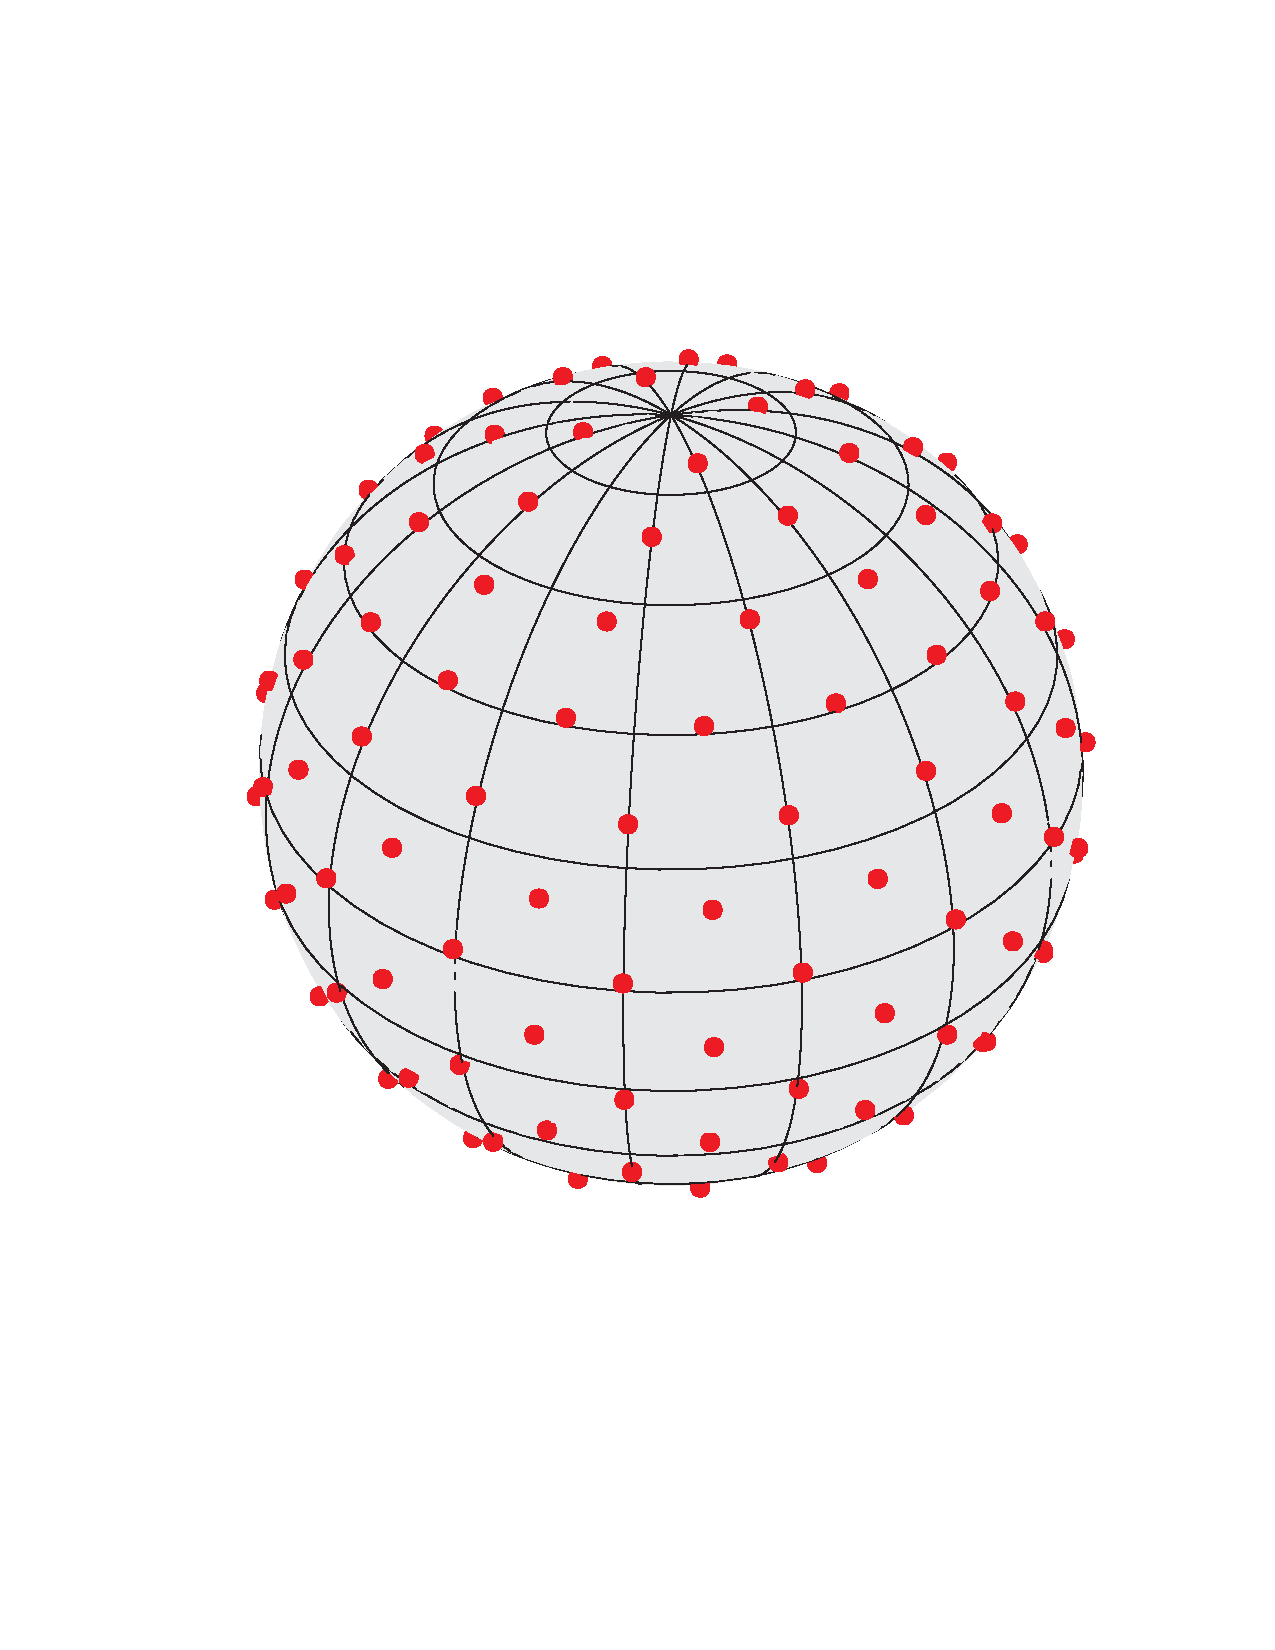
\includegraphics[height=4cm]{healpix}
      \end{figure}
    }
    \only<4>
    {
      \begin{tabular}{r|r|r}
        Iteration & $\norm{r}_{2}$ & $\norm{r}_{\infty}$ \\[0.7ex] \hline
                0 &    1.191E+04 &        4.670E+02 \\
                1 &    3.541E+01 &        1.252E+01 \\
                2 &    2.263E-01 &        5.722E-02 \\
                3 &    6.257E-04 &        1.174E-04 \\
                4 &    1.694E-05 &        5.810E-06 \\
                5 &    9.676E-08 &        5.810E-06 \\
                6 &    1.083E-08 &        5.810E-06 \\
      \end{tabular}
    }  
      \end{center}
    }
  \end{example}
\end{frame}

\begin{frame}
  \Large
  \begin{center}
    Please wake up now!
  \end{center}
\end{frame}

%\section*{Summary}

%\begin{frame}
%  \frametitle<presentation>{Summary}

%  % Keep the summary *very short*.
%  \begin{itemize}
%  \item
%    The \alert{first main message} of your talk in one or two lines.
%  \item
%    The \alert{second main message} of your talk in one or two lines.
%  \item
%    Perhaps a \alert{third message}, but not more than that.
%  \end{itemize}
%  
%  % The following outlook is optional.
%  \vskip0pt plus.5fill
%  \begin{itemize}
%  \item
%    Outlook
%    \begin{itemize}
%    \item
%      Something you haven't solved.
%    \item
%      Something else you haven't solved.
%    \end{itemize}
%  \end{itemize}
%\end{frame}

%

%% All of the following is optional and typically not needed. 
%\appendix
%\section<presentation>*{\appendixname}
%\subsection<presentation>*{For Further Reading}

%\begin{frame}[allowframebreaks]
%  \frametitle<presentation>{For Further Reading}
%    
%  \begin{thebibliography}{10}
%    
%  \beamertemplatebookbibitems
%  % Start with overview books.

%  \bibitem{Author1990}
%    A.~Author.
%    \newblock {\em Handbook of Everything}.
%    \newblock Some Press, 1990.
% 
%    
%  \beamertemplatearticlebibitems
%  % Followed by interesting articles. Keep the list short. 

%  \bibitem{Someone2000}
%    S.~Someone.
%    \newblock On this and that.
%    \newblock {\em Journal of This and That}, 2(1):50--100,
%    2000.
%  \end{thebibliography}
%\end{frame}

\end{document}


